% ju 16-Dez-22
\documentclass[a4paper,12pt,fleqn,parskip=half]{scrartcl}
\usepackage[ngerman]{babel}
\usepackage[utf8]{inputenc}
\usepackage[T1]{fontenc}

% Schrift
%\usepackage{lmodern}
\usepackage[osf,sc]{mathpazo} 
\usepackage[scale=.9,semibold]{sourcecodepro}   
\usepackage[osf]{sourcesanspro}  

\usepackage[headsepline]{scrlayer-scrpage}
\pagestyle{scrheadings}
\clearpairofpagestyles

\usepackage[table,dvipsnames,usenames]{xcolor}
\usepackage{textcase}
\usepackage{nameref}
\usepackage{hyperref}
\usepackage{tabularx}
\usepackage{multirow}
\usepackage{multicol}
\usepackage{caption, booktabs}
\usepackage{graphicx} 
\usepackage{scrhack}    
\usepackage{url}%% Links
\usepackage[inline]{enumitem}
\usepackage{pifont}
\usepackage{eurosym}% \euro 20,-
\usepackage{amsmath}
\usepackage{amsfonts}
\usepackage{amssymb}
\usepackage{array}            % Extending the array and tabular environments
\usepackage{chngcntr}         % Change the resetting of counters
\usepackage[version=4]{mhchem}
\usepackage{stmaryrd}
\usepackage{siunitx}
\usepackage{float}
\usepackage{csquotes}
\usepackage{subcaption}
\usepackage{mathtools}
\usepackage{icomma}%Dezimaltrennzeichen
\usepackage{multimedia}%Video: \movie[externalviewer]{(video.mov)}{video.mov}
\usepackage{epstopdf}
\usepackage{footnote}
\usepackage{qrcode}% Anwendung: \qrcode[hyperlink,level=Q,version=2,height=1cm]{\website}
\usepackage{underscore}% Unterstrich ____

% PDF Dokumente einbinden
\usepackage{pdfpages}% \includepdf[pages=-]{Tabellen/Excel.pdf}
\RequirePackage{lastpage}  % Pagecounter

\addto\captionsngerman{%
\renewcommand{\figurename}{Abb.}
\renewcommand{\tablename}{Tab.}
}

% listings
\usepackage{listings}
\lstset{basicstyle=\linespread{1}\ttfamily\small,floatplacement=!htb,captionpos=t,abovecaptionskip=.5\baselineskip,belowcaptionskip=.5\baselineskip,upquote=true,showstringspaces=false,inputencoding=utf8,tabsize=4,
    	keywordstyle=\bfseries ,
	commentstyle=\color{rot5},
	stringstyle=\color{orange},
	breaklines=true,
  	postbreak=\mbox{\textcolor{black}{$\hookrightarrow$}\space},
	breakatwhitespace=false
}
\lstset{literate={á}{{\'a}}1 {é}{{\'e}}1 {í}{{\'i}}1 {ó}{{\'o}}1 {ú}{{\'u}}1 {Á}{{\'A}}1 {É}{{\'E}}1 {Í}{{\'I}}1 {Ó}{{\'O}}1 {Ú}{{\'U}}1 {à}{{\`a}}1 {è}{{\`e}}1 {ì}{{\`i}}1 {ò}{{\`o}}1 {ù}{{\`u}}1 {À}{{\`A}}1 {È}{{\'E}}1 {Ì}{{\`I}}1 {Ò}{{\`O}}1 {Ù}{{\`U}}1 {ä}{{\"a}}1 {ë}{{\"e}}1 {ï}{{\"i}}1 {ö}{{\"o}}1 {ü}{{\"u}}1 {Ä}{{\"A}}1 {Ë}{{\"E}}1 {Ï}{{\"I}}1 {Ö}{{\"O}}1 {Ü}{{\"U}}1 {â}{{\^a}}1 {ê}{{\^e}}1 {î}{{\^i}}1 {ô}{{\^o}}1 {û}{{\^u}}1 {Â}{{\^A}}1 {Ê}{{\^E}}1 {Î}{{\^I}}1 {Ô}{{\^O}}1 {Û}{{\^U}}1 {œ}{{\oe}}1 {Œ}{{\OE}}1 {æ}{{\ae}}1 {Æ}{{\AE}}1 {ß}{{\ss}}1 {ű}{{\H{u}}}1 {Ű}{{\H{U}}}1 {ő}{{\H{o}}}1 {Ő}{{\H{O}}}1 {ç}{{\c c}}1 {Ç}{{\c C}}1 {ø}{{\o}}1 {å}{{\r a}}1 {Å}{{\r A}}1 {€}{{\EUR}}1 {£}{{\pounds}}1 {~}{{\textasciitilde}}1 {-}{{-}}1 }

% bibliography
\usepackage[
    bibencoding=utf8,
    backend=biber,% bibtex, biber
    backref=false,backrefstyle=three+,url=true,urldate=comp,abbreviate=false,maxnames=20
]{biblatex} %Paket laden
\DeclareBibliographyCategory{cited}
\let\defaultcite\cite\renewcommand*\cite[2][]{\addtocategory{cited}{#2}\defaultcite[#1]{#2}}
\let\defaulttextcite\textcite\renewcommand*\textcite[2][]{\addtocategory{cited}{#2}\defaulttextcite[#1]{#2}}
\setcounter{biburllcpenalty}{7000}
\setcounter{biburlucpenalty}{8000}
\AfterPackage{biblatex}{
	\PreventPackageFromLoading[\errmessage{Sie haben versucht, das Cite-Paket zu laden, das nicht mit biblatex kompatibel ist.}]{cite}
}

\hypersetup{%
	%pdftitle={\titel},
	%pdfsubject={Latex},
	%pdfauthor={\autor},
	%pdfcreator={\autor}, 
	bookmarksnumbered=true,
	breaklinks=true,
	%colorlinks=true,	   
	linkcolor=rot5,		
	filecolor=blau5,		
	urlcolor=blau5,			
	citecolor=ForestGreen
}

\linespread{1.1}
\setlist{itemsep=0pt}
\widowpenalty10000
\clubpenalty10000
\tolerance1000   

\usepackage[left=2cm,right=2cm,top=1cm,bottom=1cm,includeheadfoot]{geometry}
%\usepackage[left=4cm,right=2cm,top=1cm, bottom=1cm,includeheadfoot]{geometry}
%\usepackage[left=6cm,right=1cm,top=1cm, bottom=1cm,includeheadfoot]{geometry}
%\usepackage[landscape=true,left=2cm,right=2cm,top=1cm,bottom=1cm,includeheadfoot]{geometry}%quer

% eigene Farbe definieren
% Adobe Prozessfarben: CMYK: 100,50,0,35 -> 1,0.5,0,0.35
\definecolor{orange}{cmyk}{0,0.55,0.61,0}   % 0,55,61,0
\definecolor{blau5}{cmyk}{1,0.77,0.1,0.01}  % 100,77,10,
\definecolor{rot5}{cmyk}{0.22,1,1,0.19}     % 22,100,100,19
\definecolor{grau2}{cmyk}{0,0,0,0.1}        % 0,0,0,40
\definecolor{blau}{cmyk}{0.93,0.66,0,0.21}% 

% Literatur
\bibliography{content/literatur}
\bibliography{content/literatur-kfz}
\bibliography{content/literatur-sport}

%%%%%%%%%%%%%%%%%%%%%%%%%%%%%%%%%%%%%%%%%%%%%%%%%%%%%%%
\newcommand{\name}{Jan Unger}
\newcommand{\thema}{05-Datenbus}
\newcommand{\quelle}{\name}
\newcommand{\website}{https://bw-ju.de/}
\newcommand{\github}{https://github.com/ju1-eu}
%%%%%%%%%%%%%%%%%%%%%%%%%%%%%%%%%%%%%%%%%%%%%%%%%%%%%%%

\ihead{\textbf{Quelle:} \quelle}%{Kopfzeile innen}
\ohead{\textbf{Datum:} \today}  %{Kopfzeile außen}
\ifoot{\textbf{Thema:} \thema}  %{Fußzeile  innen}
\ofoot{Seite {\thepage} von {\pageref{LastPage}}}%{Fußzeile  außen}

\title{\thema}
\author{\name}
\date{\today}

\begin{document}
	%%%%%%%%%%%%%%%%%%%%%%%%%%%%%%%%%%%%%%%%%%%%%%%%%%%%%%%%%%%%%%%%%%
	\begin{abstract}
		\center
		\textbf{\Large \thema}%14pt
		
		\vspace{1.5em}
		%\datum	
		%\qrcode[hyperlink,level=Q,version=2,height=1cm]{\website}
		\qrcode[hyperlink,level=Q,version=2,height=1cm]{\github}
		
		\vspace{1.5em} 
		\raggedright
		\textbf{\large Keywords}
		% Checkliste
		\begin{itemize}[label=\checkmark]
			\item Begriff
		\end{itemize}
	\end{abstract}
    %%%%%%%%%%%%%%%%%%%%%%%%%%%%%%%%%%%%%%%%%%%%%%%%%%%%%%%%%%%%%%%%%%

	% anpassen
	%\input{content/tex/neu}
	%ju 17-Sep-22 05-Datenbus.tex
Quelle: Fabian Lindenberg, Kfz-Technik einfach erklärt \footnote{\url{https://www.youtube.com/watch?v=0a33FFpn_eM\&list=PLJXzCsL6HEwzoI3j8tGLKUHjLx0gTxus8}}

\textbf{Früher} für jedes Signal eine Leitung $\to$ viele Kabel
notwendig, wenn mehrere Steuergeräte auf Sensordaten zugreifen wollen.

\textbf{Heute} ein Steuergerät liest die Sensordaten aus und schickt
diese auf den Datenbus. \emph{Beispiel} Motordrehzahlsignal wird von
folgenden Steuergeräten benötigt: Motor, Getriebe, Kombiinstrument,
Klimaanlage, ESP.

\textbf{Datenübertragung im Kfz} Ermöglicht den Transport und Austausch
von Informationen in Form von Daten und Signalen.

\textbf{Gateway} ermöglicht und überwacht den Datenaustausch zwischen
Datenbussysteme mit unterschiedlichen Übertragungsgeschwindigkeiten.

\textbf{Vorteile}

\begin{enumerate}
\item
  gemeinsame Nutzung von Sensoren
\item
  verbesserte Diagnosefähigkeit
\item
  weniger elektrische Leitungen
\item
  weniger Fehlerquellen
\end{enumerate}

\section{Datenbusarten}\label{datenbusarten}

\begin{enumerate}
\item
  \textbf{elektrische Einleiter - Datenbussysteme}: LIN (Local
  Interconnect Network, Master-Slave), Multiplex

  \begin{itemize}
  \item
    Übertragungsart: elektrische Leitung
  \end{itemize}
\item
  \textbf{elektrische Zweileiter - Datenbussysteme}: CAN (Controller
  Area Network), Flexray, Ethernet

  \begin{itemize}
  \item
    Übertragungsart: elektrische Leitung
  \end{itemize}
\item
  \textbf{optische Datenbussysteme}: Glasfaser, MOST

  \begin{itemize}
  \item
    Übertragungsart: Lichtwellen
  \end{itemize}
\item
  \textbf{drahtlose Datenbussysteme}: WLAN, Bluetooth

  \begin{itemize}
  \item
    Übertragungsart: Funkwellen (elektromagnetische Wellen, 2,4 GHZ / 5
    GHz)
  \end{itemize}
\end{enumerate}

\newpage

\section{Datenbusstrukturen - Topologie -
Netzwerkstruktur}\label{datenbusstrukturen-topologie-netzwerkstruktur}

\begin{enumerate}
\item
  \textbf{Sternstruktur:} (Gateway / Router $\leftrightarrow$ PC /
  Handy / Tablet / Drucker usw.)

  \begin{itemize}
  \item
    \textbf{aktiv} (Ein Steuergerät im Zentrum eine sternförmig
    aufgebauten Datennetzes ist über Punkt-zu-Punkt-Verbindungen mit dem
    benachbarten Steuergerät verbunden.), \textbf{passiv}
    (Leitungsknoten in der Mitte)
  \end{itemize}
\item
  \textbf{Daisy-Chain:} Steuergeräte sind wie die Glieder einer Kette
  aneinander gereiht. (Gateway $\to$ PC $\to$ PC $\to$ PC $\to$
  TV)
\item
  \textbf{Busstruktur / Linear:} CAN-Bus (Datenbusleitung, Knotenpunkte,
  $SG_1 \Longleftrightarrow SG_2 \Longleftrightarrow SG_3 \Longleftrightarrow SG_n$)
\item
  \textbf{Ringstruktur} (Most) Nachteil: Bei fehlerhaften
  Lichtwellenleiter oder Steuergerät fällt die gesamte Kommunikation
  aus.
\item
  \textbf{Hybrid} (mehrere Busse)
\item
  \textbf{Maschen}
\end{enumerate}

\emph{Bemerkung:} Datenbusleitungen sind miteinander verdrillt (twisted
pair), um elektromagnetische Auswirkungen von einem auf den anderen
Draht zu minimieren. Durch die gegensätzliche Spannungsänderung heben
sich die bei jeder Umschaltung entstehenden Magnetfelder beide Leitungen
gegenseitig auf. Die Leitungen sind nach außen elektromagnetisch
neutral. (\textbf{EMV} Elektromagnetischen Verträglichkeit)

\begin{figure}[!ht]% hier: !ht
\centering
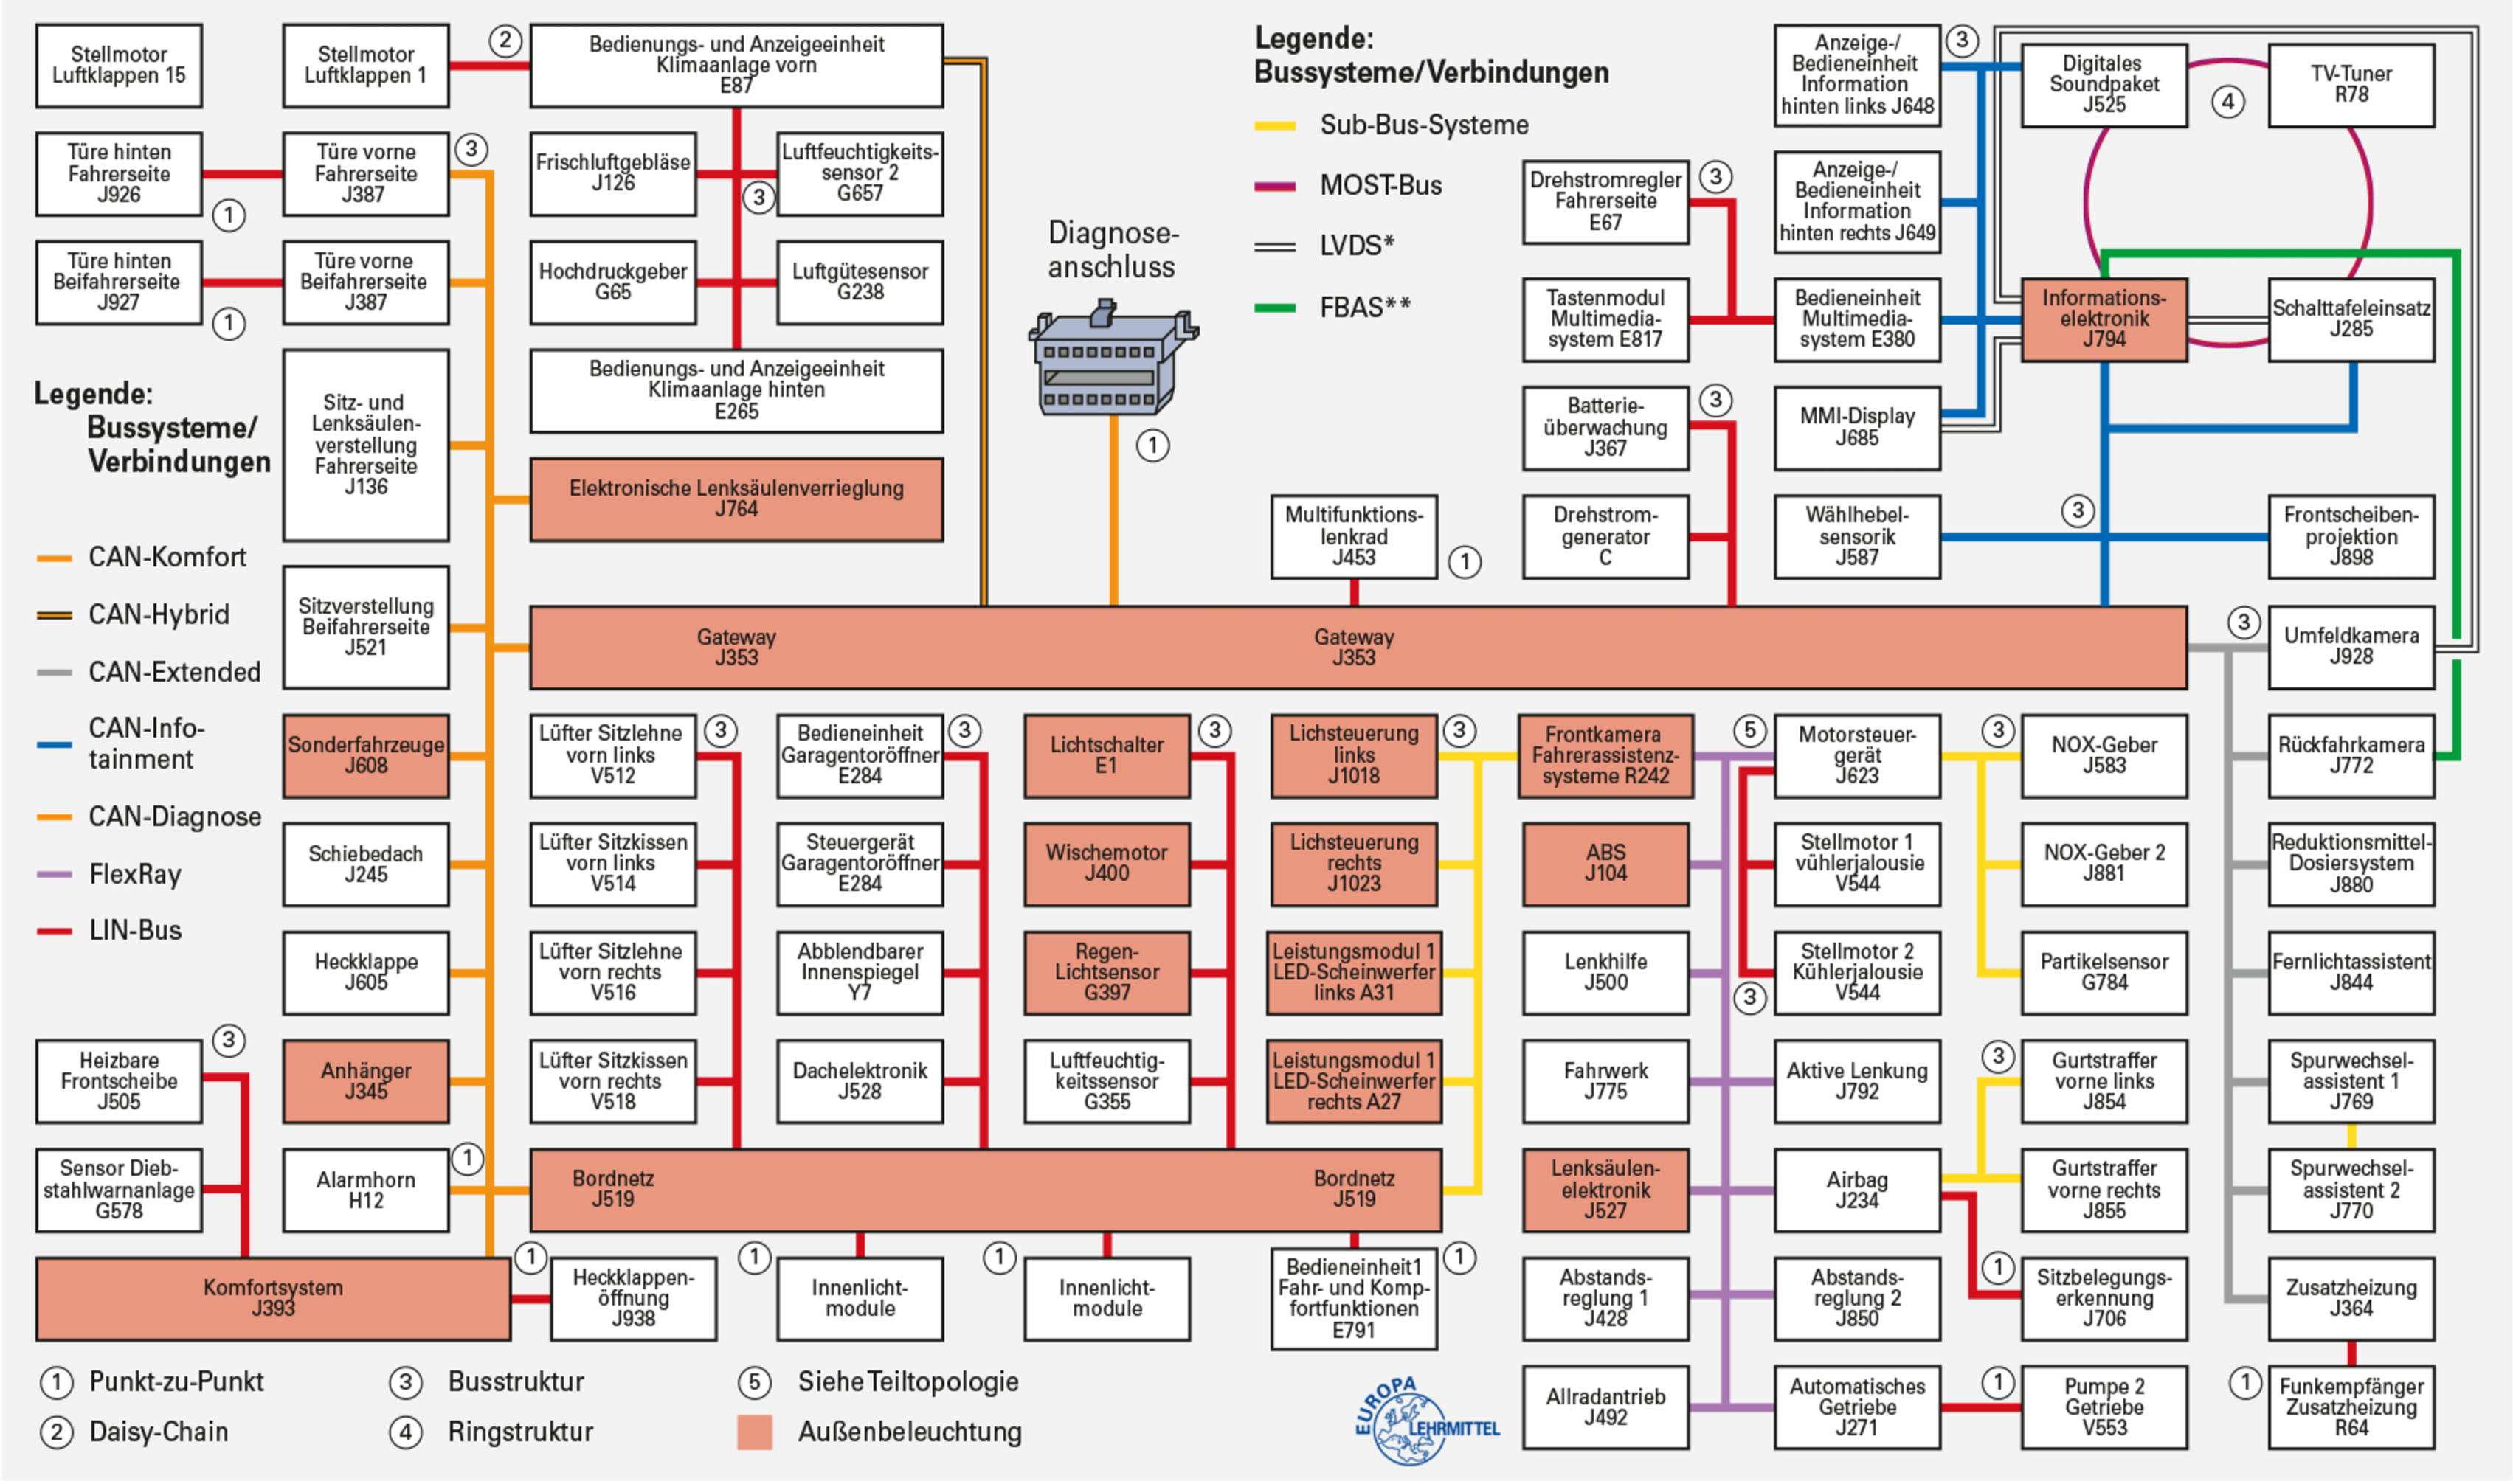
\includegraphics[width=0.9\textwidth]{images/CAN/Topologie-Datennetzwerk-Gesamtfahrzeug.png}
\caption{Topologie-Datennetzwerk-Gesamtfahrzeug, Quelle: Europa-Verlag
SimKfz}
%\label{fig:}%% anpassen
\end{figure}

\newpage

\section{CAN Klassen}\label{can-klassen}

\begin{enumerate}
\item
  \textbf{CAN Class B} (Lowspeed)

  \begin{itemize}
  \item
    bis ca. 125 kbit/s
  \item
    \textbf{Eindrahtfähig} wenn die Datenkommunikation gegeben ist, auch
    wenn eine Busleitung ausfällt
  \item
    keine Abschlusswiderstände
  \item
    \textbf{Dominant 0} low: 1 V und high: 4 V
  \item
    \textbf{Rezessiv 1} low: 5 V und high: 0 V
  \end{itemize}
\item
  \textbf{CAN Class C} (Highspeed)

  \begin{itemize}
  \item
    bis ca. 1 Mbit/s
  \item
    Nicht Eindrahtfähig
  \item
    Abschlusswiderstände $2\text{x } 60~\Omega$
  \item
    \textbf{Dominant 0} low: 1,5 V und high: 3,5 V
  \item
    \textbf{Rezessiv 1} low: 2,5 V und high: 2,5 V
  \end{itemize}
\item
  \textbf{CAN FD} (Flexible Data)

  \begin{itemize}
  \item
    bis ca. 8 Mbit/s
  \item
    Erst wenn die Daten kommen, wird die Geschwindigkeit hoch
    geschaltet.
  \end{itemize}
\end{enumerate}

\textbf{Multi-Master} Alle Steuergeräte sind gleichberechtigt. Regelung
erfolgt nach Priorität.

\textbf{Autonomes Fahren} Drive-by-Wire (alle sicherheitsrelevanten
Bauteile sind zweifach ausgelegt und zwei Bussysteme)

\newpage

\section{Aufbau CAN-Bus}\label{aufbau-can-bus}

Steuergerät sendet Nachricht auf den Datenbus.

\begin{figure}[!ht]% hier: !ht
\centering
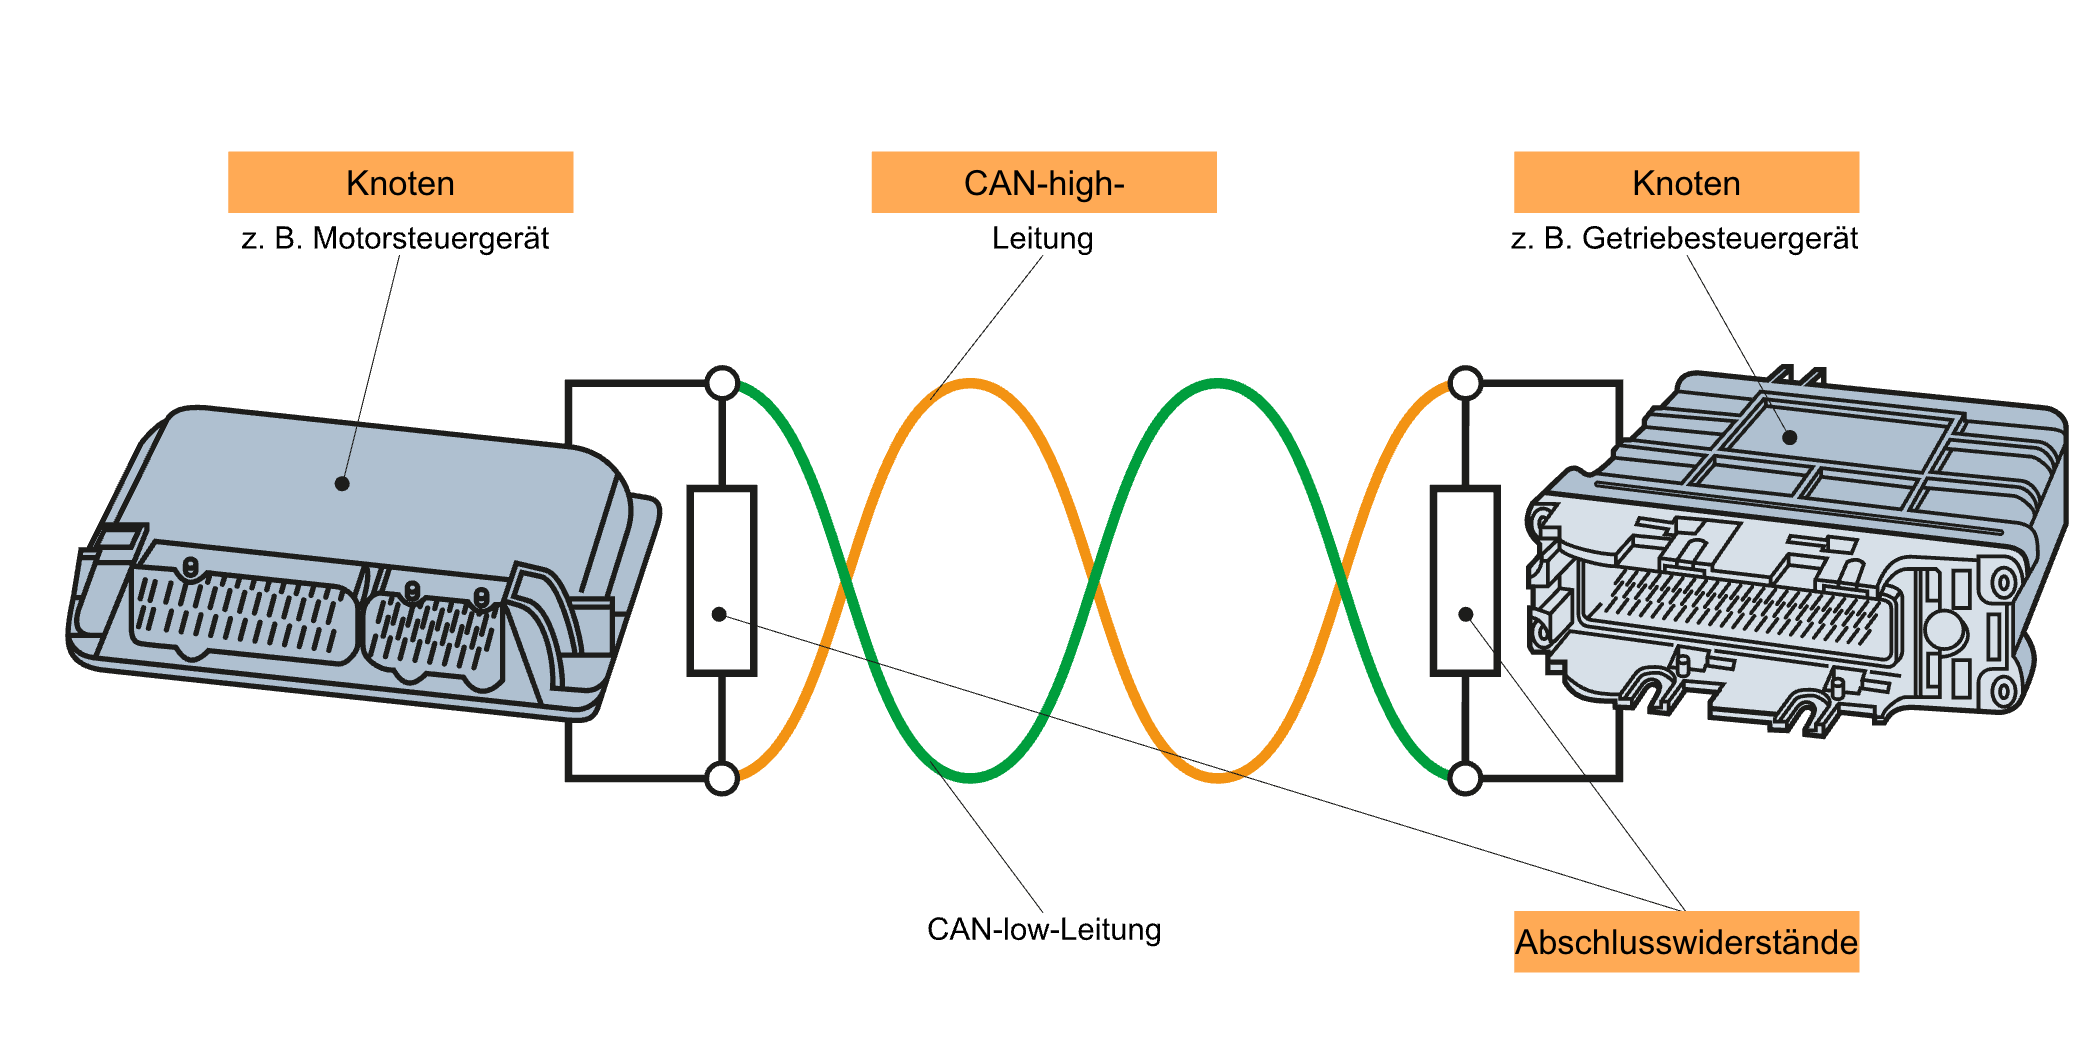
\includegraphics[width=0.6\textwidth]{images/CAN/Aufbau-CAN-Datenbus.png}
\caption{Aufbau CAN-Datenbus, Quelle: Europa-Verlag SimKfz}
%\label{fig:}%% anpassen
\end{figure}

\begin{figure}[!ht]% hier: !ht
\centering
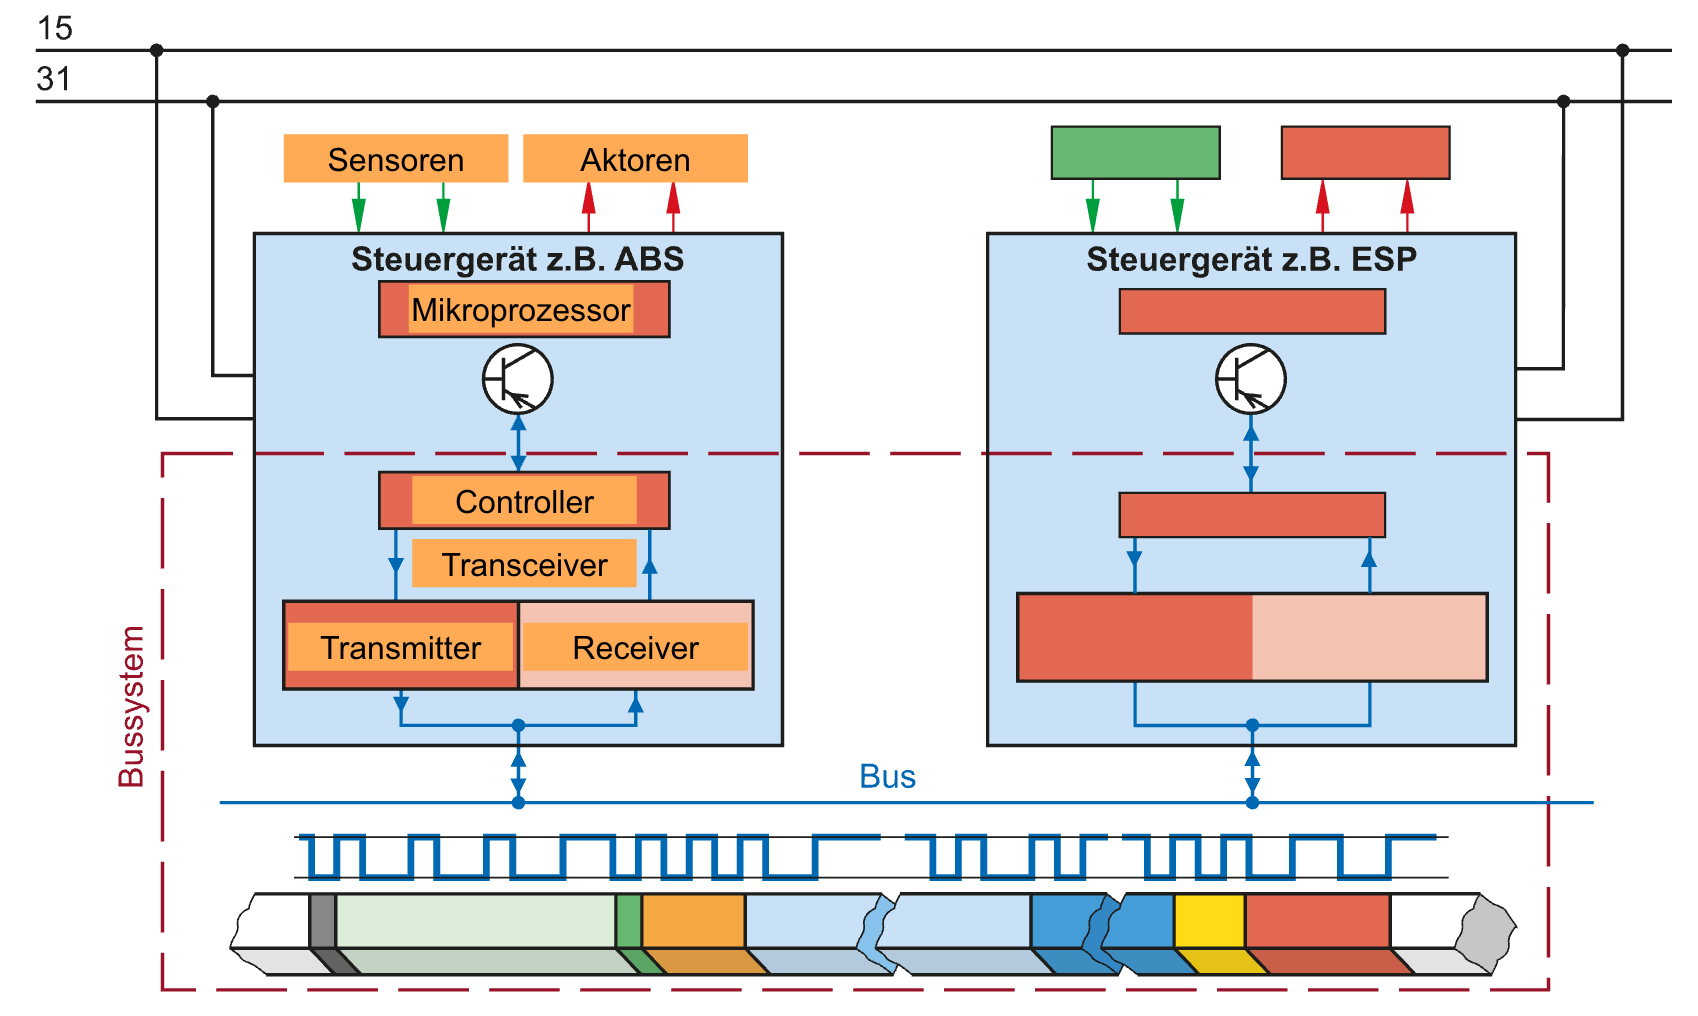
\includegraphics[width=0.6\textwidth]{images/CAN/Aufbau-elektrisches-CAN-Datenbussystem.png}
\caption{Aufbau-elektrisches-CAN-Datenbussystem, Quelle: Europa-Verlag
SimKfz}
%\label{fig:}%% anpassen
\end{figure}

\textbf{Steuergerät} (Knoten, Busteilnehmer)

\begin{enumerate}
\item
  \textbf{Microprozessor} verarbeitet die eingehenden Informationen,
  berechnet die Funktionen und steuert die Aktoren.
\item
  \textbf{Controller} filtert die für das Steuergerät notwendigen Daten
  und übermittelt sie dem Mikroprozessor.
\item
  \textbf{Transceiver} empfängt und sendet die Daten auf der Busleitung.
  Transmitter (Sender), Receiver (Empfänger)
\end{enumerate}

Beim CAN-Bussystem werden die Informationen durch Spannungsänderungen in
der Datenleitung übertragen. Dadurch empfangen alle Steuergeräte
gleichzeitig die Informationen. Die Bits werden nacheinander übertragen
(seriell).

Zwei Leitungen

\begin{enumerate}
\item
  \textbf{High-Leitung} Beim Wechsel von rezessiven (Bit = 1) zum
  dominanten (Bit = 0) Pegel steigt die Spannung.
\item
  \textbf{Low-Leitung} Beim Wechsel vom rezessiven (Bit = 1) zum
  dominanten (Bit = 0) Pegel sinkt die Spannung.
\end{enumerate}

\textbf{CAN-Buspegel}

\begin{figure}[!ht]% hier: !ht
\centering
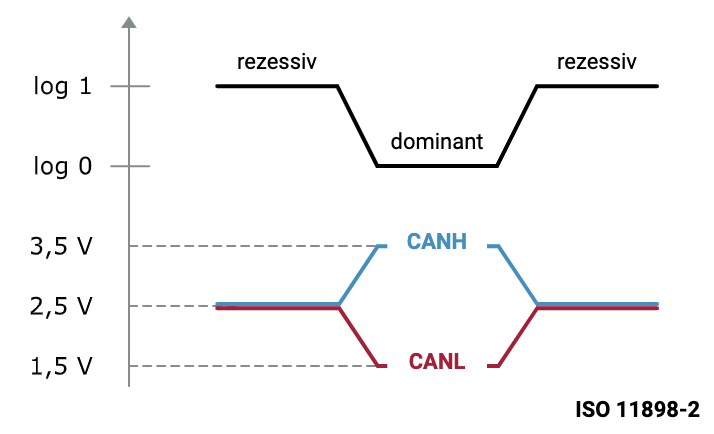
\includegraphics[width=0.4\textwidth]{images/CAN/CAN-Highspeed-Buspegel.png}
\caption[CAN-Highspeed-Buspegel, Quelle: ]{CAN-Highspeed-Buspegel,
Quelle: \footnotemark{}}
%\label{fig:}%% anpassen
\end{figure}
\footnotetext{\url{https://elearning.vector.com/mod/page/view.php?id=42}}

\begin{figure}[!ht]% hier: !ht
\centering
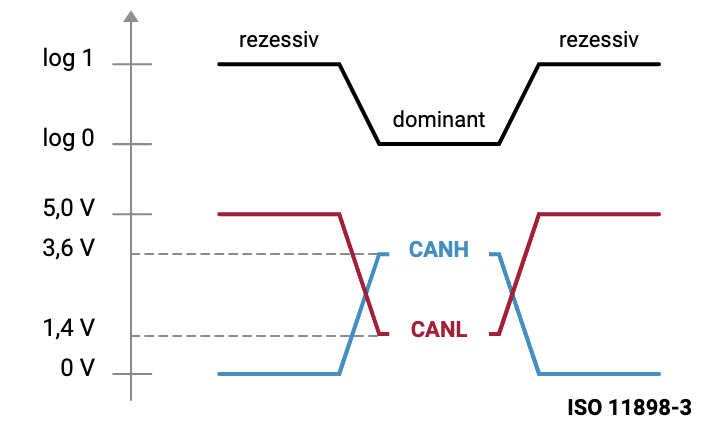
\includegraphics[width=0.4\textwidth]{images/CAN/CAN-Lowspeed-Buspegel.png}
\caption[CAN-Lowspeed-Buspegel, Quelle: ]{CAN-Lowspeed-Buspegel, Quelle:
\footnotemark{}}
%\label{fig:}%% anpassen
\end{figure}
\footnotetext{\url{https://elearning.vector.com/mod/page/view.php?id=42}}

\newpage

\section{Aufbau CAN-Nachricht -
Datenprotokoll}\label{aufbau-can-nachricht-datenprotokoll}

\begin{figure}[!ht]% hier: !ht
\centering
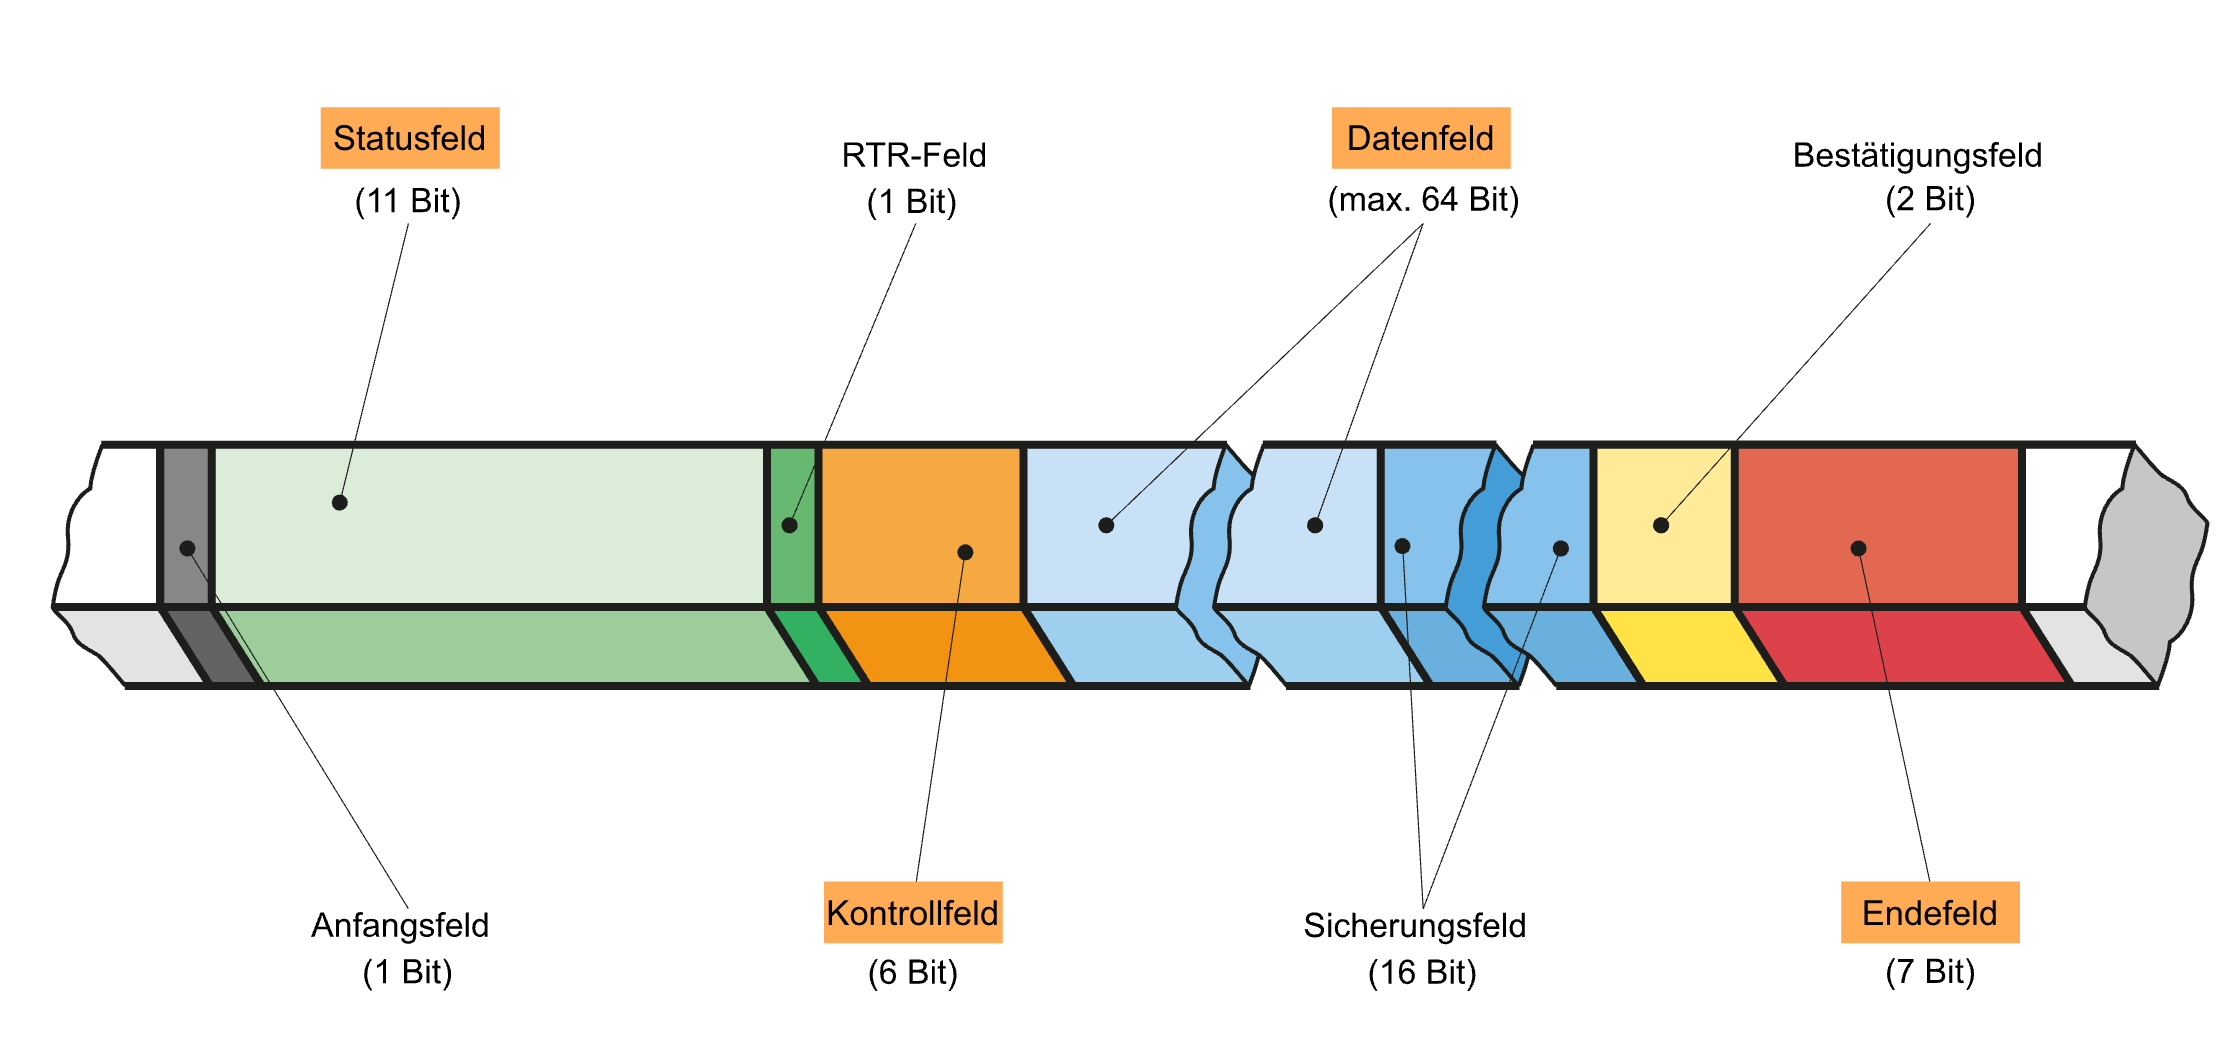
\includegraphics[width=0.6\textwidth]{images/CAN/Aufbau-CAN-Botschaft.png}
\caption{Aufbau CAN-Botschaft, Quelle: Europa-Verlag SimKfz}
%\label{fig:}%% anpassen
\end{figure}

\begin{enumerate}
\item
  Anfangsfeld (1 Bit)

  \begin{itemize}
  \item
    Beginn der Botschaft
  \end{itemize}
\item
  Statusfeld (11 Bit) Identifier

  \begin{itemize}
  \item
    Botschaftsname (Beispiel: Motordaten)
  \item
    Je niedriger die Zahl, desto wichtiger die Nachricht.
  \item
    höchste Priorität vs.~geringste Priorität
  \item
    wichtige Daten vs.~weniger wichtige Daten
  \end{itemize}
\item
  RTR (1 Bit) Remote Transmission Request Feld

  \begin{itemize}
  \item
    \textbf{0} Senden und \textbf{1} Gib mir Daten
  \end{itemize}
\item
  Kontrollfeld (6 Bit)

  \begin{itemize}
  \item
    Enthält Prüfsumme
  \end{itemize}
\item
  Datenfeld (max. 64 Bit)

  \begin{itemize}
  \item
    Motordrehzahl, Motormoment, Motortemperatur usw.
  \end{itemize}
\item
  Sicherungsfeld (16 Bit)
\item
  Bestätigungsfeld (2 Bit)
\item
  Ende (7 Bit)

  \begin{itemize}
  \item
    der Nachricht, Bus wieder frei
  \end{itemize}
\end{enumerate}

\newpage

\section{Binärzahlen umwandeln}\label{binaerzahlen-umwandeln}

\textbf{Was ist die kleinste Informationseinheit bei der
Datenübertragung?} Bit

\textbf{Wie viele Informationen können mit einem Bit übertragen werden?}
Es können zwei Informationen übertragen werden.

\lstset{language=Python}% C, TeX, Bash, Python 
\begin{lstlisting}[
	%caption={}, label={code:}%% anpassen
]
// Beispiel: 8 bit = 256 (Anzahl der Informationen)
1 Bit = 0,1 2^1 = 2
2 Bit = 00,01,10,11 2^2 = 4
3 Bit = 000,001,011,111,110,100,101,010 2^3 = 8
1 Byte = 8 bit
2^8 = 256
2^16 = 65536 
\end{lstlisting}

\textbf{Zweier Potenzen}

$2^0 = 1 \\ 2^1 = 2 \\2^2 = 4 \\2^3 = 8 \\2^4 = 16 \\2^5 = 32 \\2^6 = 64 \\2^7 = 128 \\2^8 = 256$

\textbf{Binär in Dezimal}

\lstset{language=Python}% C, TeX, Bash, Python 
\begin{lstlisting}[
	%caption={}, label={code:}%% anpassen
]
 1 0 1 1 1 // Binärzahl (5-stellig)
16 8 4 2 1 // 2-Potenz
16 0 4 2 1 // Addieren
__________
Dezimal: 23
\end{lstlisting}

\textbf{Dezimal in Binär}

\lstset{language=Python}% C, TeX, Bash, Python 
\begin{lstlisting}[
	%caption={}, label={code:}%% anpassen
]
Dezimal: 99
Test 99 < 128        // also 7-stellige Binärzahl
64 32 16  8  4  2  1 // 2-Potenz
64+32                // Addieren
96             +2 +1 
 1  1  0  0  0  1  1 // Binärzahl 
\end{lstlisting}

\newpage

\section{Fehler am CAN-Bus}\label{fehler-am-can-bus}

Messung am OBD-Stecker direkt machen.

\textbf{Messpunkte} CAN-High (Pin6) und CAN-Low (Pin14)

\textbf{Gutbild} (CAN-Low-Signal \& CAN-High-Signal sind
spiegelverkehrt)

\begin{figure}[!ht]% hier: !ht
\centering
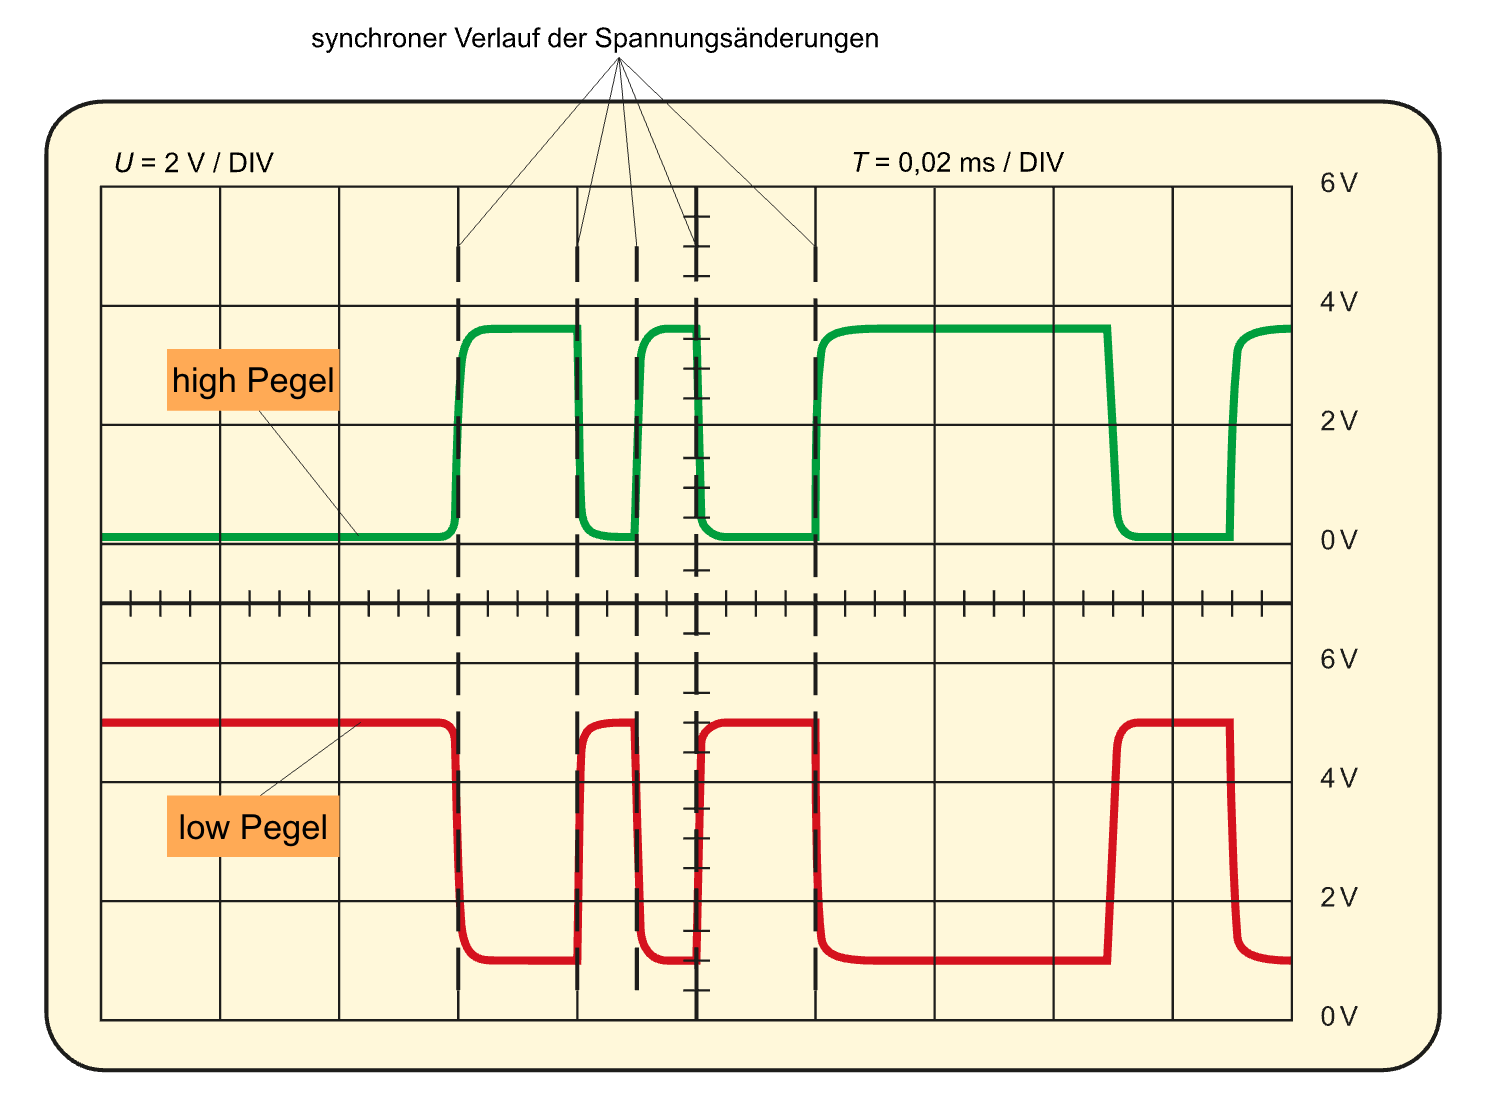
\includegraphics[width=0.4\textwidth]{images/CAN/Fehlerfreies-Signal-CAN-Bus.png}
\caption{Fehlerfreies Signal CAN-Bus, Quelle: Europa-Verlag SimKfz}
%\label{fig:}%% anpassen
\end{figure}

\begin{figure}[!ht]% hier: !ht
\centering
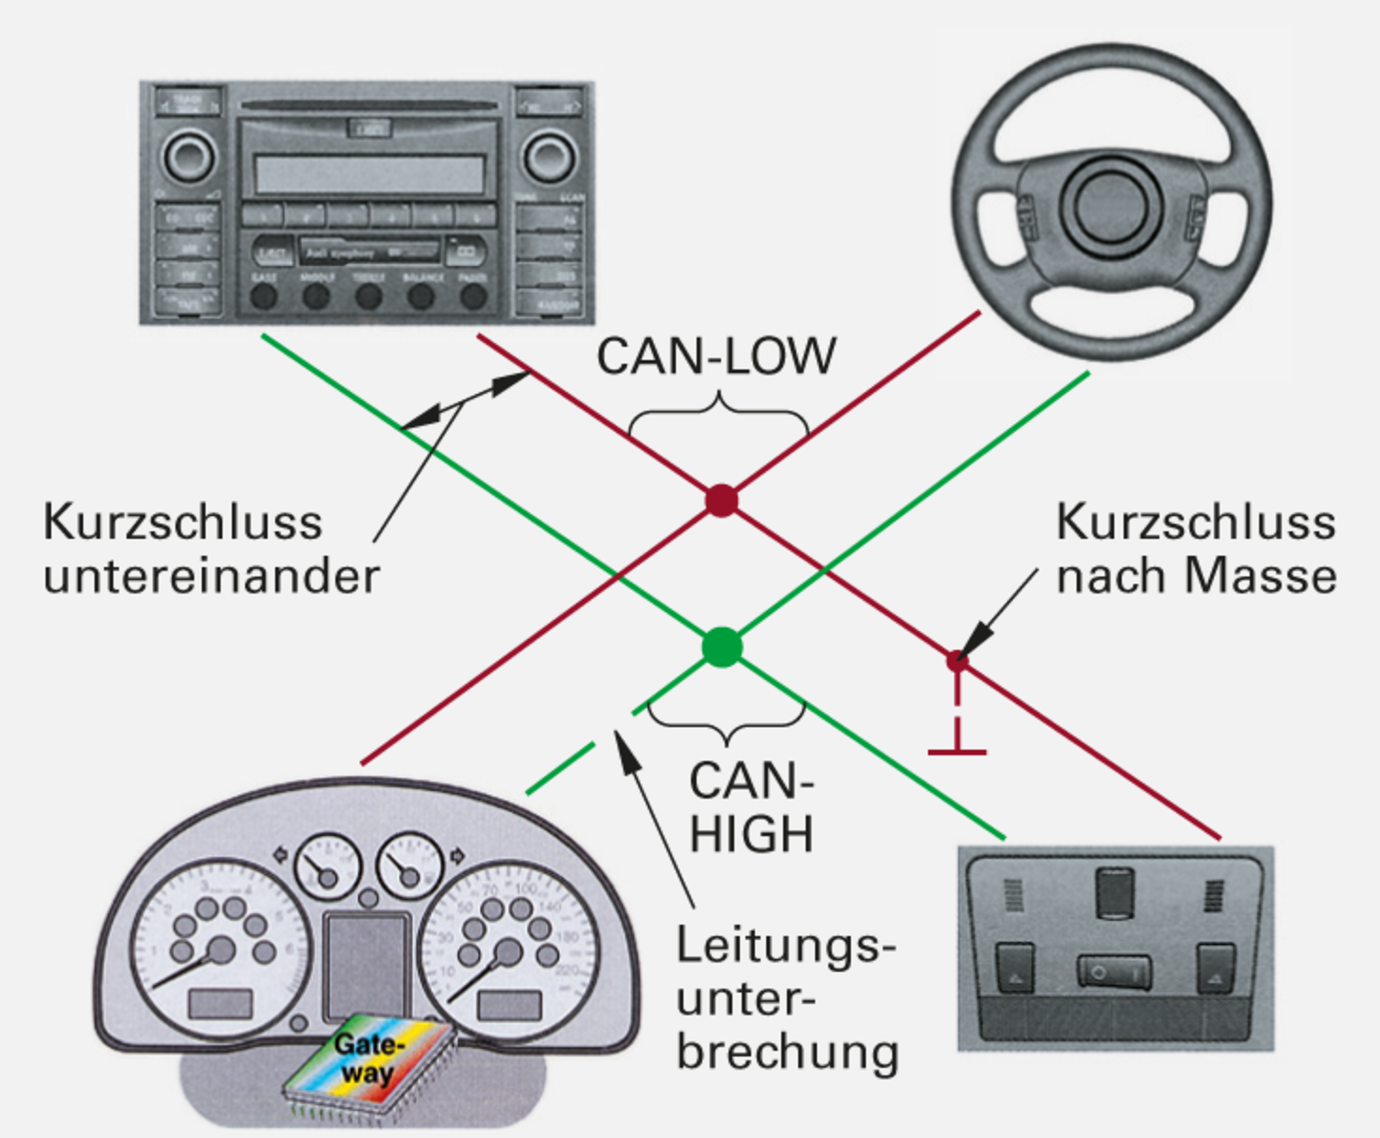
\includegraphics[width=0.4\textwidth]{images/CAN/Fehlermoeglichkeiten-CAN-Bus.png}
\caption{Fehlermöglichkeiten CAN-Bus, Quelle: Europa-Verlag SimKfz}
%\label{fig:}%% anpassen
\end{figure}

\begin{figure}[!ht]% hier: !ht
\centering
\includegraphics[width=0.8\textwidth]{images/CAN/Fehler-CAN-Bus.png}
\caption{Fehler CAN-Bus, Quelle: Europa-Verlag Arbeitsblätter
Kfz-Technik Lernfeld 9-14}
%\label{fig:}%% anpassen
\end{figure}

\newpage

\subsection{Keine Kommunikation zum SG
möglich}\label{keine-kommunikation-zum-sg-moeglich}

\begin{enumerate}
\item
  CAN-High überprüfen

  \begin{itemize}
  \item
    \textbf{Messpunkt:} Oszi an (Pin6 \& Masse)
  \end{itemize}
\item
  CAN-Low überprüfen

  \begin{itemize}
  \item
    \textbf{Messpunkt:} Oszi an (Pin14 \& Masse)
  \end{itemize}
\end{enumerate}

\textbf{kein Spannungsverlauf?}

\begin{itemize}
\item
  Beide Leitungen durchmessen
\item
  CAN-High (SG gegen Masse)
\item
  CAN-Low (SG gegen Masse)
\end{itemize}


	%%%%%%%%%%%%%%%%%%%%%%%%%%%%%%%%%%%%%%%%%%%%%%%%%%%%%%%%%%%%%%%%%%
    % Bibliographie
    \printbibliography[category=cited]
\end{document}
